\documentclass{standalone}
\usepackage{tikz}
\usepackage{bm}
\usetikzlibrary{fit,positioning}
\usepackage{
    algorithm,algorithmic,amsfonts,amsmath,amssymb,bm,booktabs,color,
    enumerate,graphicx,hyperref,microtype,multicol,natbib,nicefrac,url
}
\usepackage[T1]{fontenc}
\usepackage[utf8]{inputenc}

\newcommand{\todo}[1]{\noindent\textbf{\textcolor{red}{(TODO) #1\\}}}

\newcommand{\MDP}{M}
\newcommand{\States}{\mathcal{S}}
\newcommand{\Actions}{\mathcal{A}}
\newcommand{\cost}{C}
\newcommand{\initstatedist}{\rho}
\newcommand{\discount}{\gamma}
\newcommand{\numsamp}{N}
\newcommand{\horizon}{T}
\newcommand{\dynamics}{p}
\newcommand{\policyparams}{\theta}
\newcommand{\policy}{\pi}
\newcommand{\state}{\mathbf{s}}
\renewcommand{\action}{\mathbf{a}}
\newcommand{\costsample}{c}
\newcommand{\policyobj}{\eta}
\newcommand{\dynmodel}{\hat{\dynamics}}
\newcommand{\costmodel}{\hat{\cost}}
\newcommand{\isdmodel}{\hat{\rho}}
\newcommand{\dynmat}{\mathbf{F}}
\newcommand{\dyncovar}{\Sigma}
\newcommand{\costmat}{\mathbf{C}}
\newcommand{\costvec}{\mathbf{c}}
\newcommand{\K}{\mathbf{K}}
\renewcommand{\k}{\mathbf{k}}
\newcommand{\polcovar}{\mathbf{S}}
\newcommand{\latent}{\mathbf{x}}
\newcommand{\traj}{\tau}
\newcommand{\polstepsize}{\epsilon_p}
\newcommand{\modelstepsize}{\epsilon_m}
\newcommand{\R}{\mathbb{R}}
\newcommand{\N}{\mathcal{N}}
\newcommand{\W}{\mathcal{W}}
\renewcommand{\L}{\mathcal{L}}
\newcommand{\E}{\mathbb{E}}
\newcommand{\I}{\mathbb{I}}
\newcommand{\KL}{\text{KL}}
\newcommand{\model}{\mathcal{M}}
\newcommand{\dataset}{\mathcal{D}}
\DeclareMathOperator*{\argmin}{argmin}
\DeclareMathOperator*{\argmax}{argmax}
\newcommand{\colvec}[2][.67]{%
  \scalebox{#1}{%
    \renewcommand{\arraystretch}{.67}%
    $\begin{bmatrix}#2\end{bmatrix}$%
  }
}
\newcommand{\trajectory}{\left[\state_0,\action_0,\ldots,\state_\horizon,\action_\horizon,\state_{\horizon + 1}\right]}
\newcommand{\costtrajectory}{\left[\state_0,\action_0,\costsample_0\ldots,\state_\horizon,\action_\horizon,\costsample_\horizon,\state_{\horizon + 1}\right]}
\newcommand{\latenttrajectory}{\left[\latent_0,\action_0,\ldots,\latent_\horizon,\action_\horizon,\latent_{\horizon + 1}\right]}

\begin{document}
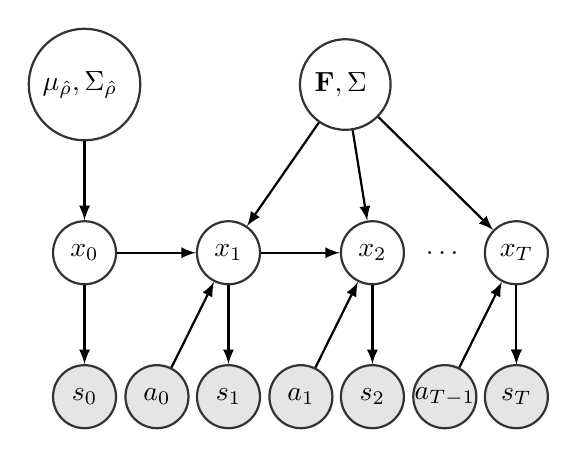
\begin{tikzpicture}
\tikzstyle{main}=[circle, minimum size = 8mm, thick, draw =black!80, node distance = 20mm]
\tikzstyle{connect}=[-latex, thick]
\tikzstyle{box}=[rectangle, draw=black!100]
    %\state_0~|~\mu_{\isdmodel},\Sigma_{\isdmodel}&\sim\N(\mu_{\isdmodel}, \Sigma_{\isdmodel})\,,~~~~~\state_{t+1}~|~\state_t,\action_t&&\sim\N\left(\dynmat\begin{bmatrix}\state_t\\\action_t\end{bmatrix},\dyncovar\right) \textrm{ for } t \in [0,\ldots,\horizon]
  \node[main, align=center] (p) [] { $\mu_{\isdmodel}, \Sigma_{\isdmodel}$ };
  \node[main, align=center] (F) [right=of p] { $\dynmat,\dyncovar$ };
  \node[main] (x0) [below=1cm of p] { $x_0$ };
  \node[main] (x1) [right=1cm of x0] { $x_1$ };
  \node[main] (x2) [right=1cm of x1] { $x_2$ };
  \node[main] (xT) [right=1cm of x2] { $x_T$ };
  \node[main, fill=black!10] (s0) [below=1cm of x0] { $s_0$ };
  \node[main, fill=black!10] (s1) [below=1cm of x1] { $s_1$ };
  \node[main, fill=black!10] (s2) [below=1cm of x2] { $s_2$ };
  \node[main, fill=black!10] (sT) [below=1cm of xT] { $s_T$ };
  \node[main, fill=black!10] (a0) [left=0.08cm of s1] { $a_0$ };
  \node[main, fill=black!10] (a1) [left=0.08cm of s2] { $a_1$ };
  \node[main, inner sep=0pt, fill=black!10] (aT_1) [left=0.08cm of sT] { $a_{T - 1}$ };
  %\node[main] (theta) [right=of z] { $\bm{\mu}$ };
  %\node[main, fill = black!10] (f) [below=of z] { $x_{i}$ };
  \path (p) edge [connect] (x0)
        (a0) edge [connect] (x1)
        (a1) edge [connect] (x2)
        (x0) edge [connect] (x1)
        (x1) edge [connect] (x2)
        (x0) edge [connect] (s0)
        (x1) edge [connect] (s1)
        (x2) edge [connect] (s2)
        (xT) edge [connect] (sT)
        (xT) edge [connect] (sT)
        (F) edge [connect] (x1)
        (F) edge [connect] (x2)
        (F) edge [connect] (xT)
        (aT_1) edge [connect] (xT)
        (x2) -- node[auto=false]{\ldots} (xT)
        ;
  %\node[rectangle, inner sep=0mm, fit= (f),label=below right:D, xshift=-1mm, yshift=1mm] {};
  %\node[rectangle, inner sep=4.4mm,draw=black!100, fit= (f)] {};
  %\node[rectangle, inner sep=4.6mm, fit= (z) (f),label=below right:N, xshift=-1mm, yshift=-12mm] {};
  %\node[rectangle, inner sep=9mm, draw=black!100, fit = (z) (f)] {};
\end{tikzpicture}
\end{document}
